% !TeX root = ../tesis.tex

\chapter{Introducción}
\label{ch:introduccion}

Debido al crecimiento demográfico exponencial, la Ciudad de México enfrenta
desafíos estructurales complejos, entre los cuales destaca la movilidad
intraurbana y metropolitana como el eje central de la presente investigación.
Esta problemática tiene raíces históricas profundas; si bien desde el Porfiriato
el automóvil fue concebido como un símbolo de modernidad, su consolidación como
eje de la planeación urbana ocurrió entre las décadas de 1920 y 1930. Durante
este periodo, la expansión urbana y la motorización transformaron aceleradamente
la morfología de la capital \citep{franco2022}.

En consecuencia, durante la segunda mitad del siglo XX, se priorizó un modelo de
ciudad volcado hacia el autotransporte mediante la construcción de arterias
viales para vehículos particulares y de carga. Este desarrollo de
infraestructura y servicios de transporte público fue el factor determinante en
la ubicación y conectividad de los nuevos fraccionamientos con el centro de la
ciudad \citep{franco2022}.

En este contexto, la dinámica de movilidad respondió a la constante necesidad de
desplazamiento entre distintos puntos de la capital. Una consecuencia directa de
ello fue la construcción de vialidades de mayor capacidad para sostener el
creciente volumen de traslados, lo cual propició, a su vez, la expansión de la
mancha urbana en sus dimensiones habitacional, laboral y de servicios.

\begin{quote}
``Entre éstas destacaron la Avenida de los Insurgentes, que se extendió hasta el
municipio de San Ángel como parte de los festejos del centenario de la
consumación de la Independencia en 1921 [\ldots] Hacia el norte, sobre la
Calzada de Guadalupe se construyeron barrios populares y para trabajadores
industriales, tales como las colonias Maza, Peralvillo, Valle Gómez, Vallejo y
del Rastro.'' \citep[p.~XX]{franco2022}
\end{quote}

Sin embargo, todo este avance de movilidad tuvo su auge para las rutas
concesionadas de camiones y transportes motorizados. A diferencia de los
tranvías, cuya implementación implicaba mayores costos y tiempos de instalación,
los camiones concesionados ofrecieron mayor versatilidad y cobertura
\citep{franco2022}.

Las carreteras representaron la principal vía de comunicación por toda la
república mexicana. Este crecimiento urbano evidenció la necesidad de ampliar y
robustecer las vialidades, derivando en la expansión de la mancha urbana.
Diversos estudios han señalado que las carreteras fungen como catalizadores de
nuevos desarrollos urbanos \citep{garcia2019allroads}. Según
\citet{garcia2019allroads}, las autopistas expanden las ciudades con mayor
desarrollo urbanístico y reducen su densidad residencial general, generando
nuevos desarrollos más discontinuos, fragmentados, rodeados de terreno sin
urbanizar y más aislados de otras áreas artificiales (traducción propia).

De este mismo texto podemos extraer una de las figuras que da estructura a
nuestra investigación: los patrones espaciales alternativos de desarrollo de
suelo en el proceso de suburbanización de la población, representados en tres
figuras: \textit{Compact, linear} y \textit{leapfrog} (Compacto, lineal y
saltón). Según \citet{jia2010}, pueden distinguirse tres patrones espaciales de
desarrollo urbano: el desarrollo saltón muestra mayor fragmentación y
aislamiento; el lineal implica menor fragmentación pero mayor aislamiento; y el
compacto, aunque más eficiente, también puede derivar en expansión si la
densidad residencial disminuye (traducción propia).

\begin{figure}[htbp]
    \centering
    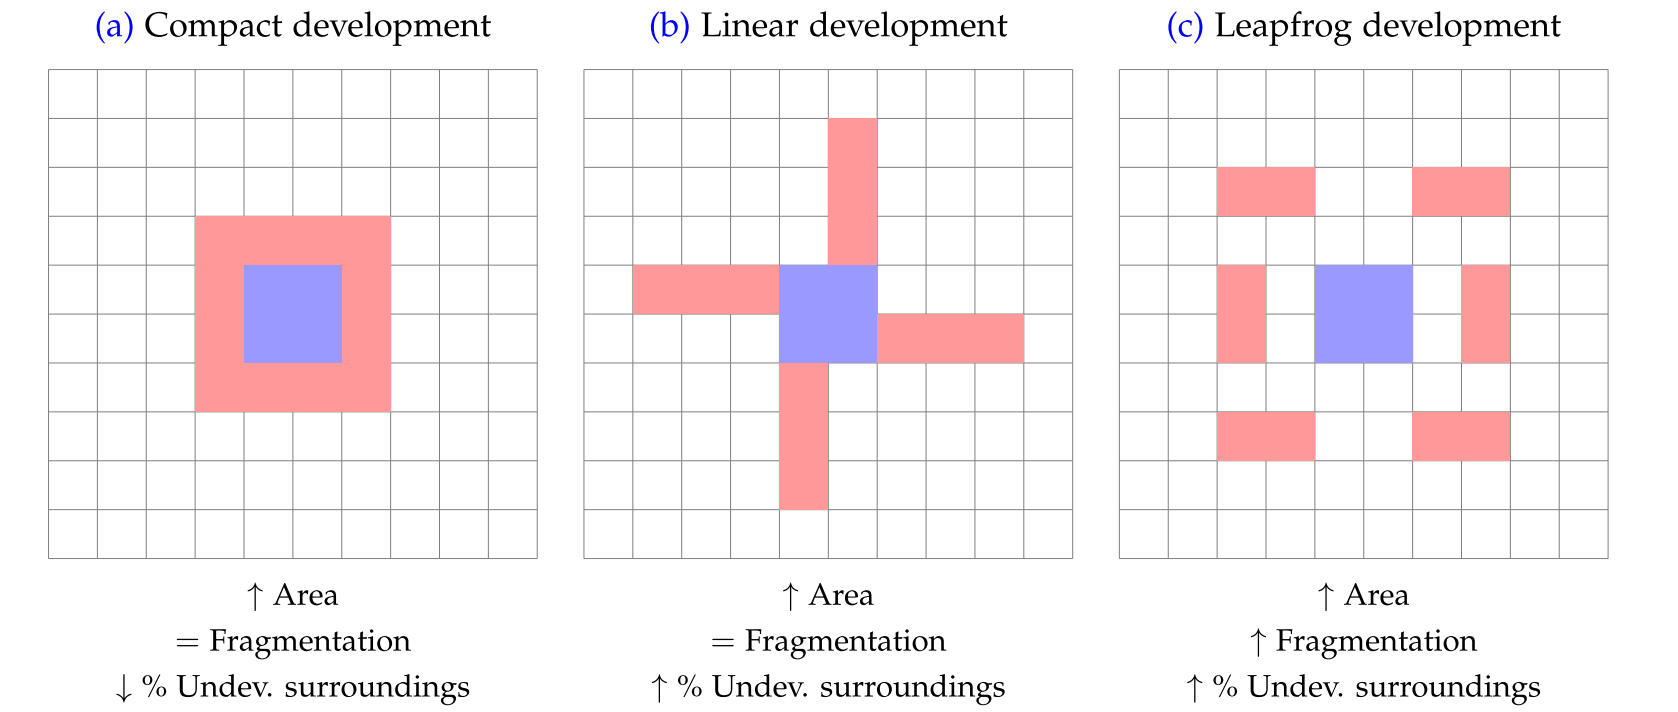
\includegraphics[width=0.85\textwidth]{Figures/Cap1/Sprawl}
    \caption[Patrones de desarrollo urbano]{Patrones espaciales de desarrollo de suelo:
compacto, lineal y saltón (\textit{Compact, Linear and Leapfrog development}).}
    \label{fig:sprawl}
    \small\textit{Fuente: García-López (2019, p.~3).}
\end{figure}

En el caso de la Ciudad de México, la expansión en colonias del sur y oriente a
lo largo de ejes como Tlalpan o Periférico Sur corresponde a un patrón lineal;
mientras que los nuevos desarrollos en Milpa Alta y Tláhuac muestran rasgos de
patrón saltón, al estar aislados de la mancha urbana consolidada.

En este marco, la presente investigación propone una metodología replicable para
cuantificar las vulnerabilidades funcionales de la red de transporte multimodal
de la \zmvm{} y evaluar el impacto topológico de escenarios alternativos de alta
capacidad, tomando los cuatro cuadrantes del Anillo Periférico de la \cdmx{}
como caso hipotético de demostración.

%-----------------------------------------------------------------------
\section{Problemática}
\label{sec:problematica}
%-----------------------------------------------------------------------

El Periférico de la Ciudad de México fue concebido como una infraestructura
estratégica para conectar diversos puntos de la capital. Indirectamente, creó
los límites más visibles para la ciudad, ocasionando la centralización de
actividades comerciales, legislativas y, en particular, de transporte. Con el
paso de los años, algunas zonas han experimentado crecimientos acelerados
producto del desbordamiento poblacional, haciendo más notoria la ausencia de
transporte público masivo en distintas secciones del anillo. Las alcaldías más
afectadas son Xochimilco, Milpa Alta, Tláhuac y Tlalpan, que carecen de opciones
de traslados de alta capacidad y dependen principalmente de transporte
concesionado como camiones y vagonetas, además del uso intensivo del automóvil
particular.

Esta situación responde, en buena medida, a la falta histórica de inversión en
transporte público, lo que ha fomentado el uso individualizado del automóvil y
disminuido la eficiencia del sistema de movilidad en su conjunto. Tal como
señalan especialistas en movilidad urbana \citep{cano2002}, el impacto del
transporte motorizado se refleja en un incremento del tráfico, de modo que la
construcción o ampliación de vialidades urbanas solo ofrece una solución
temporal: al cabo de tres a cinco años, estas nuevas infraestructuras tienden a
saturarse por el aumento de viajes inducidos.

